%   % !TEX root = ../../VIII,3_Rahmen-TeX_9-0.tex
%  
%   Band VIII, 3 N.~?? 	[STO??.?]			
%   Signatur/Tex-Datei:	LH_37_05_144r
%   RK-Nr. 	57267_1
%   Datierung:		März 1677 (a. St.)
%   WZ: 	Bl. 145 Mitte, Nr. 803005
%   edlabels:			3		
%   Diagramme: 		6 					
%
%
%
\selectlanguage{ngerman}
\frenchspacing
%
\begin{ledgroupsized}[r]{120mm}
\footnotesize
\pstart
\noindent\textbf{Überlieferung:}
\pend
\end{ledgroupsized}
%
\begin{ledgroupsized}[r]{114mm}
\footnotesize
\pstart \parindent -6mm
\makebox[6mm][l]{\textit{L}}%
Konzept:
LH~XXXVII~5~Bl.~144\textendash145. %ggf. (unsere Druckvorlage).
Ein Bogen~2\textsuperscript{o};
Wasserzeichen in der Mitte von Bl.~145;
Papiererhaltungsmaßnahmen;
Papierbruch an den Blatträndern mit geringfügigem Textverlust.
Eine Seite auf Bl.~144~r\textsuperscript{o}.
Auf Bl.~144~v\textsuperscript{o} und 145~r\textsuperscript{o} sowie im Randbereich von Bl.~144~r\textsuperscript{o} wird N.~\ref{57267_2} überliefert.
Die unteren zwei Drittel von Bl.~145~r\textsuperscript{o} und der obere Rand von Bl.~145~v\textsuperscript{o} überliefern N.~\ref{57267_3}.
Bl.~145~v\textsuperscript{o} und der untere linke Bereich von Bl.~144~v\textsuperscript{o} überliefern N.~\ref{57268}.
\pend
\end{ledgroupsized}
%
\begin{ledgroupsized}[r]{114mm}
\footnotesize
\pstart
\parindent -6mm
\makebox[6mm][l]{\textit{E}}%
(tlw.) \textsc{Fichant} 1994, S.~356f.\cite{01056}
\pend%
\end{ledgroupsized}
%
%
\selectlanguage{latin}
\frenchspacing
% \newpage%
\vspace{8mm}
\pstart%
\normalsize%
\noindent%
\lbrack144~r\textsuperscript{o}\rbrack\
\pend
%
\pstart
\noindent
\raggedleft
Martii 1677
\pend
\count\Bfootins=1100%
\count\Afootins=1100%
\count\Cfootins=1100
%
\pstart\noindent
\hspace{1mm}\hspace{-1mm}% Trick, weil \edlabel nicht zu \par-Beginn sein darf
%
\edlabel{37_05_144r_1a}%
\edtext{}{% ergänzung (3 Absätze)
{\xxref%
{37_05_144r_1a}{37_05_144r_1b}}%
\lemma{}%
\Bfootnote{%
Regulae \lbrack...\rbrack\ derivemus. \textit{erg.}~\textit{L}%
}}%
Regulae duae:
\pend
%
\pstart
(1) Eadem
%
\edtext{est potentia corporum\protect\index{Sachverzeichnis}{potentia}}{\lemma{est}\Bfootnote{\textit{(1)}~vis \textit{(2)}~potentia \textit{(a)}~ante et post concursum \textit{(b)}~corporum~\textit{L}}}
%
ante et post concursum\protect\index{Sachverzeichnis}{concursus}. 
\pend
%
\pstart
(2) Centrum gravitatis\protect\index{Sachverzeichnis}{centrum gravitatis} corporum aequaliter procedit%
\protect\index{Sachverzeichnis}{centrum gravitatis aequaliter procedens}
ante et post concursum.\protect\index{Sachverzeichnis}{concursus} Seu eadem est directio 
aggregati corporum\protect\index{Sachverzeichnis}{aggregatum corporum}%
\protect\index{Sachverzeichnis}{directio aggregati corporum} ante et post concursum.\protect\index{Sachverzeichnis}{concursus}
\pend
%
\pstart
Ex his reliqua derivemus.\edlabel{37_05_144r_1b}
\pend 
%
\vspace{1.5em} %%%%%%%%% Diagramm 1
\centerline{%
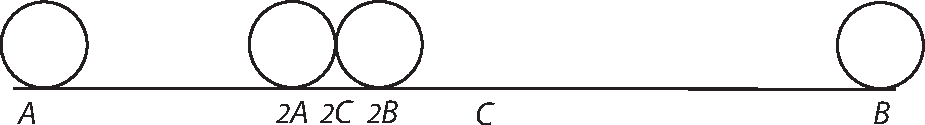
\includegraphics[width=0.7\textwidth]{%
gesamttex/edit_VIII,3/images/LH_37_05_144r_d1.pdf%
}} 
\vspace{0.5em}
\centerline{%
\lbrack\textit{Fig.~1}\rbrack%
}
% \newpage%
%\vspace{1.5em}
%
%
\vspace{1.5em} %%%%%%%%% Diagramm 2
\centerline{%
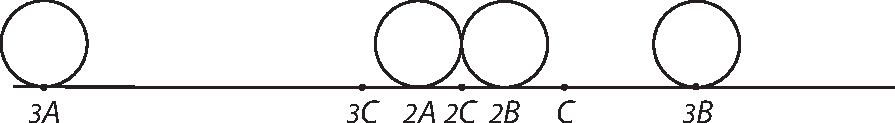
\includegraphics[width=0.7\textwidth]{%
gesamttex/edit_VIII,3/images/LH_37_05_144r_d2.pdf%
}} 
\vspace{0.5em}
\centerline{%
\lbrack\textit{Fig.~2}\rbrack%
}
% \newpage%
\vspace{1.2em}
%
\pstart
Sint duo corpora aequalia%
\protect\index{Sachverzeichnis}{corpora aequalia} \textit{A}, \textit{B},
concurrentia celeritatibus inaequalibus%
\protect\index{Sachverzeichnis}{celeritates inaequales} \textit{A{\scriptsize2}A}, \textit{B{\scriptsize2}B}. %
Centrum gravitatis\protect\index{Sachverzeichnis}{centrum gravitatis} eorum erit in
medio distantiae \textit{C}, nempe ita ut sint \textit{AC} et \textit{BC} aequales. Concursu%
\protect\index{Sachverzeichnis}{concursus} translatum erit in \textit{{\scriptsize2}C},
adeoque %
via centri gravitatis\protect\index{Sachverzeichnis}{via centri gravitatis} erit \textit{C{\scriptsize2}C}. Post concursum%
\protect\index{Sachverzeichnis}{concursus} intellegimus nihilominus centrum
gravitatis\protect\index{Sachverzeichnis}{centrum gravitatis} aequaliter procedere%
\protect\index{Sachverzeichnis}{centrum gravitatis aequaliter procedens} in \textit{{\scriptsize3}C}, et esse \textit{{\scriptsize2}C{\scriptsize3}C} aequ.\ \textit{C{\scriptsize2}C}. 
%
Quaeruntur loca jam 
%
\edtext{in qu\lbrack ae\rbrack\ \textit{A}}{\lemma{in}\Bfootnote{\textbar\ quibus \textit{ändert Hrsg.} \textbar\ %
\textit{(1)}~consistent \textit{(2)}~\textit{A}~\textit{L}}}
%
et \textit{B} 
%
\edtext{post concursum\protect\index{Sachverzeichnis}{concursus} eadem}{\lemma{concursum}\Bfootnote{\textit{(1)}~ea qua \textit{(2)}~eadem~\textit{L}}}
%
qua ad concursum\protect\index{Sachverzeichnis}{concursus} venere celeritate
deferentur, seu quaeruntur puncta ${\scriptstyle \textit{3}}A, {\scriptstyle \textit{3}}B$.
\pend
%
\pstart
Patet ante omnia \textit{{\scriptsize3}A{\scriptsize3}C} esse aequalem
ipsi \textit{{\scriptsize3}B{\scriptsize3}C}. 
\pend
%
\pstart
Patet quoque ${\scriptstyle \textit{2}}A{\scriptstyle \textit{3}}A + {\scriptstyle \textit{2}}B{\scriptstyle \textit{3}}B$ aequare debere $A{\scriptstyle \textit{2}}A \,+$ 
%
\edtext{\textit{B{\scriptsize2}B}, ex eo qui\lbrack a\rbrack\ eandem}{\lemma{\textit{B{\scriptsize2}B}}\Bfootnote{\textit{(1)}~. Ergo \textit{(2)}~, ex eo \textbar\ qui \textit{ändert Hrsg.} \textbar\ eandem~\textit{L}}}
%
 vim%
\protect\index{Sachverzeichnis}{vis} servatam esse necesse est, ac proinde eandem quantitatem celeritatum
in corpora ductarum,%
\protect\index{Sachverzeichnis}{quantitas celeritatis in corpus ductae} id est (quia corpora aequalia sunt) eandem longitudinem rectarum 
%
\edtext{percursarum. Addatur}{\lemma{percursarum.}\Bfootnote{\textit{(1)}~Ergo erit \textit{(2)}~Addatur~\textit{L}}}
%
utrobique \textit{{\scriptsize2}A{\scriptsize2}B}, fiet
%
$\underbrace{{\scriptstyle \textit{3}}A{\scriptstyle \textit{2}}A+{\scriptstyle \textit{2}}A{\scriptstyle \textit{2}}B+{\scriptstyle \textit{2}}B{\scriptstyle \textit{3}}B}_{\displaystyle{\scriptstyle \textit{3}}A{\scriptstyle \textit{3}}B} \ \sqcap$%
%
\edtext{$\underbrace{A{\scriptstyle \textit{2}}A + {\scriptstyle \textit{2}}A{\scriptstyle \textit{2}}B + {\scriptstyle \textit{2}}BB}_{\displaystyle AB}$. Quia}{\lemma{
$\underbrace{A{\scriptstyle \textit{2}}A + {\scriptstyle \textit{2}}A{\scriptstyle \textit{2}}B + {\scriptstyle \textit{2}}BB}_{\displaystyle AB}$
}\Bfootnote{\textit{(1)}~. Ergo cum detur punctum \textit{{\scriptsize3}C}, medium rectae \textit{(2)}~Quia~\textit{L}}}
%
ergo \textit{AB} et \textit{{\scriptsize3}A{\scriptsize3}B} aequantur, ergo et dimidiae,
%
\rule[0cm]{0mm}{10pt}%
\textit{AC}, \textit{{\scriptsize3}A{\scriptsize3}C}, \textit{BC}, \textit{{\scriptsize3}B{\scriptsize3}C} aequabuntur. Ergo si ex puncto \textit{{\scriptsize3}C}
dato velut centro, radio autem \textit{AC} describatur circulus\lbrack,\rbrack\ is rectam in qua corpora decurrunt
secabit in punctis \textit{{\scriptsize3}A}, \textit{{\scriptsize3}B}. Eaque proinde habentur. Hinc patet corpora \textit{AB} inter se
permutasse celeritatem.
\pend \pstart
\noindent
\begin{tabular}{llllllll}
Nam corpus &\hspace*{-3mm}\textit{A}& quod venerat in&\hspace*{-3mm}\textit{{\scriptsize2}A} &
celeritate &\hspace*{-3mm}\textit{A{\scriptsize2}A} &
redit in &\hspace*{-3mm}\textit{{\scriptsize3}A} \\
\dotfill&\hspace*{-3mm}\textit{B}&\dotfill &\hspace*{-2mm}\textit{{\scriptsize2}B}&\dotfill &\dotfill \hspace*{-3mm}\textit{B{\scriptsize2}B}&\dotfill &\dotfill \hspace*{-3mm}\textit{{\scriptsize3}B}
\\
&&celeritate &\hspace*{-3mm}\textit{{\scriptsize2}A{\scriptsize3}A} & aequali &\hspace*{-3mm}\textit{B{\scriptsize2}B}&&\\
&&\dotfill &\dotfill \hspace*{-3mm}\textit{{\scriptsize2}B{\scriptsize3}B}&\dotfill &\dotfill \hspace*{-3mm}\textit{A{\scriptsize2}A}.&&
\end{tabular}
\pend \pstart\noindent
Esse autem \textit{{\scriptsize2}A{\scriptsize3}A} aequ.\ \textit{B{\scriptsize2}B} et \textit{{\scriptsize2}B{\scriptsize3}B} aequ.\ \textit{A{\scriptsize2}A} sic demonstratur.\pend
%
 \pstart\noindent
$\left. \begin{array}{rrr} {\scriptstyle \textit{2}}A{\scriptstyle \textit{3}}A \ \textup{aequ.}\ \underbrace{{\scriptstyle \textit{3}}C{\scriptstyle \textit{3}}A}_{\displaystyle AC\; \sqcap\; BC} & + \underbrace{ {\scriptstyle \textit{2}}C{\scriptstyle \textit{3}}C}_{\displaystyle C{\scriptstyle \textit{2}}C} & - \underbrace{ {\scriptstyle \textit{2}}C{\scriptstyle \textit{2}}A}_{\displaystyle {\scriptstyle \textit{2}}C{\scriptstyle \textit{2}}B} \\
B{\scriptstyle \textit{2}}B \ \textup{aequ.}\ BC  &+ C{\scriptstyle \textit{2}}C & - {\scriptstyle \textit{2}}C{\scriptstyle \textit{2}}B \end{array} \ \ \right\}$ Ergo \textit{{\scriptsize2}A{\scriptsize3}A} aequ.\ \textit{B{\scriptsize2}B}, et eodem modo
erit 
%
\edtext{\lbrack\textit{{\scriptsize2}B{\scriptsize3}B}\rbrack}{\lemma{}\Bfootnote{\textit{{\scriptsize2}B{\scriptsize3}A}~\textit{L} \textit{ändert Hrsg.}}}
% 
aequ.\ \textit{A{\scriptsize2}A}.
\pend \pstart
Sint jam duo corpora inaequalia,%
\protect\index{Sachverzeichnis}{corpora inaequalia} \textit{A}, \textit{B}, eaque ponantur ferri celeritate aequali%
\protect\index{Sachverzeichnis}{celeritates aequales} usque ad
concursum,\protect\index{Sachverzeichnis}{concursus} quaeritur quid sit futurum post concursum\protect\index{Sachverzeichnis}{concursus}.
\pend
%
\vspace{2.0em} %%%%%%%%% Diagramm 3
\centerline{%
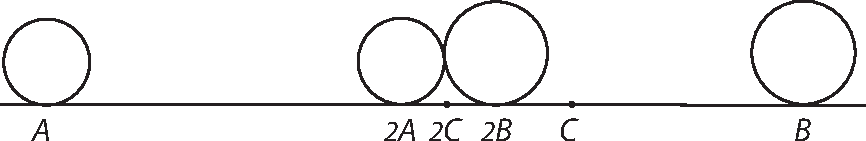
\includegraphics[width=0.7\textwidth]{%
gesamttex/edit_VIII,3/images/LH_37_05_144r_d3.pdf%
}} 
\vspace{0.5em}
\centerline{%
\lbrack\textit{Fig.~3}\rbrack%
}
\newpage%
%\vspace{1.5em}
%
%
%\vspace{2.0em} %%%%%%%%% Diagramm 4
\centerline{%
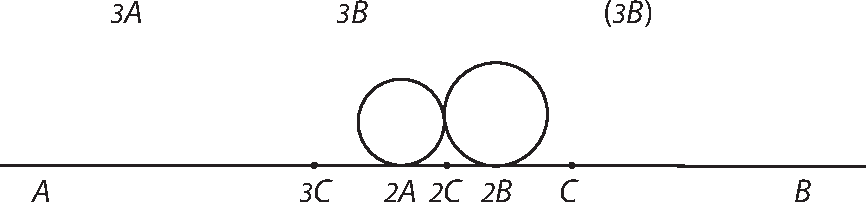
\includegraphics[width=0.7\textwidth]{%
gesamttex/edit_VIII,3/images/LH_37_05_144r_d4.pdf%
}} 
\vspace{0.5em}
\centerline{%
\lbrack\textit{Fig.~4}\rbrack%
}
% \newpage%
\vspace{2.0em}
%
%\vspace{2.0em} %%%%%%%%% Diagramm 5
\centerline{%
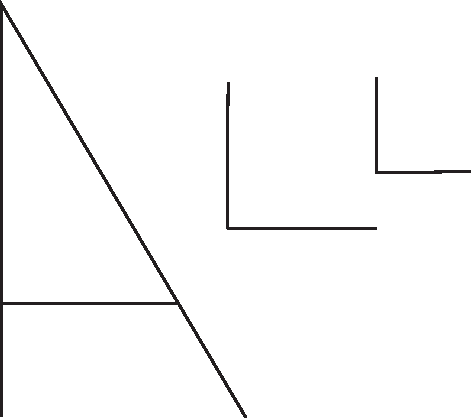
\includegraphics[width=0.33\textwidth]{%
gesamttex/edit_VIII,3/images/LH_37_05_144r_d5.pdf%
}}
\vspace{0.5em}
\centerline{%
\lbrack\textit{Fig.~5}\rbrack%
}
% \newpage%
\vspace{1.0em}

%
 \pstart
In ipsa \textit{AB} 
%
\edtext{suma\lbrack t\rbrack ur}{%
\lemma{}%
\Bfootnote{%
sumantur %
\textit{L ändert Hrsg.}%
}}
%
\textit{C}, centrum gravitatis\protect\index{Sachverzeichnis}{centrum gravitatis} corporum \textit{A}\lbrack,\rbrack\ \textit{B}, ita ut \textit{AC} sit ad \textit{BC}, ut \textit{B} ad \textit{A}. Eodem modo
habebitur punctum 
\textit{{\scriptsize2}C}, 
erit enim 
\textit{{\scriptsize2}A{\scriptsize2}C} 
ad 
\textit{{\scriptsize2}B{\scriptsize2}C}, 
ut 
\textit{B} ad \textit{A}, seu ut \textit{AC} ad \textit{BC}. 
Datis ergo punctis \textit{C} et 
\textit{{\scriptsize2}C}, 
datur
etiam punctum \textit{{\scriptsize3}C}, quia 
\textit{{\scriptsize2}C{\scriptsize3}C}, aequ.\ \textit{C{\scriptsize2}C}. 
%
\edtext{Porro potentia%
\protect\index{Sachverzeichnis}{potentia} corporum}{\lemma{Porro}\Bfootnote{\textit{(1)}~vis \textit{(2)}~potentia \textit{(a)}~ante \textit{(b)}~corporum~\textit{L}}}
%
ante
concursum%
\protect\index{Sachverzeichnis}{concursus} erat factum ex corporibus in celeritatem hoc loco communem,%
\protect\index{Sachverzeichnis}{factum ex corporibus in celeritatem communem}  et quia celeritas illa hoc loco
est 
\textit{A{\scriptsize2}A} 
vel
\textit{B{\scriptsize2}B} 
aequales, corpora vero repraesentari possunt, \textit{B} quidem recta \textit{AC}, et \textit{A} recta 
\textit{BC}. Ideoque 
%
\edtext{potentia \protect\index{Sachverzeichnis}{potentia} corporum}{\lemma{potentia}\Bfootnote{\textit{(1)}~haec reprae \textit{(2)}~corporum~\textit{L}}}
%
tota repraesentabitur per 
$AC + CB,\ \smallfrown \ 
A{\scriptstyle \textit{2}}A$ seu $AB \ \smallfrown \ B{\scriptstyle \textit{2}}B$. 
Ut ergo aequalis sit haec %
potentia\protect\index{Sachverzeichnis}{potentia} etiam post concursum\protect\index{Sachverzeichnis}{concursus}, ideo necesse 
est \textit{BC} in 
${\scriptstyle \textit{2}}A{\scriptstyle \textit{3}}A, + AC$ 
in 
\textit{{\scriptsize2}B{\scriptsize3}B} 
aequari ipsi 
\textit{AC} 
in 
\begin{tabular}[t]{cc}
 ${A{\scriptstyle \textit{2}}A},$ & $+\ CB$ \\
vel \textit{B{\scriptsize2}B} &
\end{tabular}
%$\underset{\displaystyle \textup{vel}\ B{\scriptstyle \textit{2}}B}{A{\scriptstyle \textit{2}}A}, + CB$ 
in
\begin{tabular}[t]{c}
\textit{A{\scriptsize2}A}. \\
vel \textit{B{\scriptsize2}B}
\end{tabular}
%$\underset{\displaystyle \textup{vel}\ B{\scriptstyle \textit{2}}B}{A{\scriptstyle \textit{2}}A}$. 
\pend
%
\pstart\noindent
${\scriptstyle \textit{2}}A{\scriptstyle \textit{3}}A \ \sqcap \ \underbrace{{\scriptstyle \textit{2}}C{\scriptstyle \textit{3}}C}_{\displaystyle C{\scriptstyle \textit{2}}C} +\, {\scriptstyle \textit{3}}C{\scriptstyle \textit{3}}A - {\scriptstyle \textit{2}}C{\scriptstyle \textit{2}}A$
et 
${\scriptstyle \textit{2}}B{\scriptstyle \textit{3}}B \ 
\sqcap\ 
{\scriptstyle \textit{2}}B{\scriptstyle \textit{2}}C %
\edtext{+ {\scriptstyle \textit{2}}C{\scriptstyle \textit{3}}C - {\scriptstyle \textit{3}}C{\scriptstyle \textit{3}}B$ si corpus \textit{B} progredi pergit. Est}{%
\lemma{$+ {\scriptstyle \textit{2}}C{\scriptstyle \textit{3}}C$}%
\Bfootnote{%
\textit{(1)}~\pleibdashv %
\textit{(2)}~$ -\; {\scriptstyle \textit{3}}C{\scriptstyle \textit{3}}B $ %
\textbar\ si corpus \textit{B} progredi \textit{(1)}~continuat \textit{(2)}~pergit \textit{erg.}~\textbar\ . Est
\textit{L}%
}}
%
\rule[0cm]{0mm}{12pt}%
$\displaystyle\frac{{\scriptstyle \textit{3}}C{\scriptstyle \textit{3}}B}{{\scriptstyle \textit{3}}C{\scriptstyle \textit{3}}A} \ \sqcap\ \displaystyle\frac{BC}{AC}$.
%
Ergo erit
%
${\scriptstyle \textit{3}}C{\scriptstyle \textit{3}}B \ \sqcap\ \displaystyle\frac{BC}{AC}\, {\scriptstyle \textit{3}}C{\scriptstyle \textit{3}}A$.
Unde in aequatione praecedenti 
\rule[0cm]{0mm}{12pt}%
explicando
%
\textit{{\scriptsize2}A{\scriptsize3}A}, \textit{{\scriptsize2}B{\scriptsize3}B}, \textit{{\scriptsize3}C{\scriptsize3}B}
fiet:
%
$C{\scriptstyle \textit{2}}C \smallfrown BC,+ {\scriptstyle \textit{3}}C{\scriptstyle \textit{3}}A \smallfrown BC,\, - 
\underbrace{{\scriptstyle \textit{2}}C{\scriptstyle \textit{2}}A \smallfrown 
BC,,\, + {\scriptstyle \textit{2}}B{\scriptstyle \textit{2}}C \smallfrown AC,}_{\displaystyle \sqcap\ 0} \,+ C{\scriptstyle \textit{2}}C \smallfrown AC,\, - \displaystyle\frac{BC}{\ovalbox{\textit{AC}}}\, {\scriptstyle \textit{3}}C{\scriptstyle \textit{3}}A \smallfrown \ovalbox{\textit{AC}} \ \sqcap \ AC \smallfrown A{\scriptstyle \textit{2}}A,\, +
%
\edtext{CB \smallfrown$ \textit{A{\scriptsize2}A}. At}{\lemma{$CB \smallfrown$ \textit{A{\scriptsize2}A}.}\Bfootnote{\textit{(1)}~Quod si jam \textit{(a)}~$\leibdashv$ \textit{(aa)}~\textit{BC} \textit{(bb)}~${\scriptstyle \textit{3}}$ \textit{(cc)}~$BC \ \sqcap$ \textit{(b)}~fiet \textit{{\scriptsize3}C} \textit{(2)}~At~\textit{L}}}
%
\rule[0cm]{0mm}{12pt}%
${\scriptstyle \textit{3}}C{\scriptstyle \textit{3}}A \smallfrown BC$ destruetur et restabit 
$C{\scriptstyle \textit{2}}C \smallfrown \underset{\displaystyle AC}{BC}\ \sqcap\ A{\scriptstyle \textit{2}}A \smallfrown \underset{\displaystyle BC}{ AC}\ \underset{\displaystyle \,\textup{vel}\, \ B{\scriptstyle \textit{2}}B}{ \,\textup{seu}\, \ A{\scriptstyle \textit{2}}A}\ \sqcap\ C{\scriptstyle \textit{2}}C$. 
\rule[0cm]{0mm}{12pt}%
Quod est absurdum, nam si $B{\scriptstyle \textit{2}}B\ \sqcap C{\scriptstyle \textit{2}}C$ erit ${\scriptstyle \textit{2}}B{\scriptstyle \textit{2}}C\ \sqcap BC$ quod est absurdum. 
%
\pend 
\pstart
Huic absurditati non licet aliter mederi, quam   
%
\edtext{faciendo ut \textit{{\scriptsize2}B} non pergat, sed regrediatur. Quod ut fiat punctum \textit{{\scriptsize3}B} sumendum in contrariam partem, ita erit}{%
\lemma{faciendo}%
\Bfootnote{%
\textit{(1)}~$ \pleibdashv\; \sqcap\; + $ seu ${\scriptstyle \textit{2}}B{\scriptstyle \textit{3}}B \sqcap {\scriptstyle \textit{2}}B{\scriptstyle \textit{2}}C + {\scriptstyle \textit{2}}C{\scriptstyle \textit{3}}C + {\scriptstyle \textit{3}}C{\scriptstyle \textit{3}}B$. Quod fiet %
\textit{(a)}~si
\textit{(b)}~si
\textit{(c)}~\textit{{\scriptsize3}B} sumendo in contrariam partem, ita ut corpus \textbar\ ex \textit{erg.}~\textbar\ \textit{{\scriptsize2}B} regredi intelligitur, %
\textit{(2)}~ut \textit{{\scriptsize2}B} \lbrack...\rbrack\ erit %
\textit{L}%
}}
%
enim
%
${\scriptstyle \textit{2}}B{\scriptstyle \textit{3}}B \ \sqcap \ {\scriptstyle \textit{3}}B{\scriptstyle \textit{3}}C \ \underbrace{
- {\scriptstyle \textit{2}}C{\scriptstyle \textit{3}}C - {\scriptstyle \textit{2}}B{\scriptstyle \textit{2}}C
}_{\displaystyle -{\scriptstyle \textit{2}}B{\scriptstyle \textit{3}}C}$.
%
\pend \vspace{1mm}\pstart
Nimirum cum necessario \textit{{\scriptsize3}C} sit inter \textit{{\scriptsize3}A} et \textit{{\scriptsize3}B} quippe eorum centrum,%
\protect\index{Sachverzeichnis}{centrum} et ob impenetrabilitatem,%
\protect\index{Sachverzeichnis}{impenetrabilitas} necessario \textit{{\scriptsize3}B} maneat ad partem dextram \textit{{\scriptsize3}A} ad sinistram, ideo alterutrum necesse est\lbrack:\rbrack\ 
vel \textit{{\scriptsize3}B} cadere inter \textit{{\scriptsize3}C}
%
\edtext{et \textit{{\scriptsize2}B}, seu corpus \textit{B} progredi ex \textit{{\scriptsize2}B} in \textit{{\scriptsize3}B}\lbrack,\rbrack}{\lemma{et \textit{{\scriptsize2}B},}\Bfootnote{\textit{(1)}~et erit \textit{(2)}~seu corpus \lbrack...\rbrack\ in \textit{{\scriptsize3}B}~\textit{L}}}
%
et tunc erit 
\textit{{\scriptsize2}B{\scriptsize3}B} 
aequ.\ 
${\scriptstyle \textit{2}}B{\scriptstyle \textit{3}}C\; - $  
%
\edtext{\textit{{\scriptsize 3}B{\scriptsize 3}C}, quod}{%
\lemma{\textit{{\scriptsize 3}B{\scriptsize 3}C},}%
\Bfootnote{%
\textit{(1)}~vel %
\textit{(2)}~quod %
\textit{L}%
}}
%
absurdum parere ostendimus. Vel necesse est 
\textit{{\scriptsize2}B} 
cadere inter 
\textit{{\scriptsize3}B} 
et 
\textit{{\scriptsize3}C}, 
et
tunc 
\textit{B} 
regredietur ex 
\textit{{\scriptsize2}B} 
in 
\textit{{\scriptsize3}B}, 
fietque
%
${\scriptstyle \textit{2}}B{\scriptstyle \textit{3}}B\ \sqcap\ {\scriptstyle \textit{3}}B{\scriptstyle \textit{3}}C - {\scriptstyle \textit{2}}B{\scriptstyle \textit{3}}C$.
%
\pend \pstart
Hinc patet \edtext{\lbrack si\rbrack}{%
\lemma{}%
\Bfootnote{%
suo %
\textit{L ändert Hrsg.}%
}}
duo corpora perfecte dura%
\protect\index{Sachverzeichnis}{corpus perfecte durum} utcunque inaequalia%
\protect\index{Sachverzeichnis}{corpora inaequalia} in eadem recta sibi occurrant 
aequivelociter, necessario repelli ambo, ac proinde etiam maximum corpus%
\protect\index{Sachverzeichnis}{corpus maximum} a minimo%
\protect\index{Sachverzeichnis}{corpus minimum} aequiveloci
repelli. Jam et aequale ab aequali repellitur, si aequivelocia sunt, itaque illud generale erit:
si duo corpora aequivelociter sibi in eadem recta occurrant, ambo
%
\edtext{repellentur, atque}{\lemma{repellentur,}\Bfootnote{\textit{(1)}~ita a \textit{(2)}~atque~\textit{L}}}
%
ita
motus corporis maximi\protect\index{Sachverzeichnis}{corpus maximum} a minimo%
\protect\index{Sachverzeichnis}{corpus minimum} occurrente aequivelociter in contrarium verti potest. Quod videtur 
paradoxum,%
\protect\index{Sachverzeichnis}{paradoxum} et ab omni ratione%
\protect\index{Sachverzeichnis}{ratio} alienum, experientiae%
\protect\index{Sachverzeichnis}{experientia} quoque contrarium, in omnibus quae apud nos sunt
corporibus. Interim calculum absolvemus:
\pend
%
\pstart
\noindent
%
${\scriptstyle \textit{2}}A{\scriptstyle \textit{3}}A\ \sqcap\ {\scriptstyle \textit{2}}A{\scriptstyle \textit{3}}C + {\scriptstyle \textit{3}}C{\scriptstyle \textit{3}}A$.
%
Ergo fiet:\pend
\pstart\noindent
%
$\begin{array}{cccccc}
{\scriptstyle \textit{2}}A{\scriptstyle \textit{3}}C \smallfrown BC,\; + %
& \underbrace{{\scriptstyle \textit{3}}C{\scriptstyle \textit{3}}A} \smallfrown BC,,\; + %
& \underbrace{{\scriptstyle \textit{3}}B{\scriptstyle \textit{3}}C} \smallfrown AC,\; - %
& {\scriptstyle \textit{2}}B{\scriptstyle \textit{3}}C \smallfrown AC\ \sqcap  %
& A{\scriptstyle \textit{2}}A%
&\smallfrown AC.\\
%	\rule{0mm}{10pt}
& {\displaystyle {\scriptstyle \textit{3}}B{\scriptstyle \textit{3}}C \smallfrown \displaystyle\frac{AC}{BC}}\;\;\;\;\;\; %
& {\displaystyle {\scriptstyle \textit{3}}C{\scriptstyle \textit{3}}A \smallfrown \displaystyle\frac{BC}{AC}}\;\;\;\; %
& & 
\textup{vel}\ B{\scriptstyle \textit{2}}B%
&\;\;BC
	\end{array}$
\pend
%
\pstart\noindent Ergo 
%
${\scriptstyle \textit{3}}A{\scriptstyle \textit{3}}C 
\sqcap 
\displaystyle\frac
{
	\underset
		{
			\displaystyle \textup{\ovalbox{vel \textit{B{\scriptsize2}B}}}
		}{
			A{\scriptstyle \textit{2}}A
		} 
\smallfrown 
\underset{\displaystyle BC}{AC}\ \
\underset{\displaystyle -{\scriptstyle \textit{2}}A{\scriptstyle \textit{3}}C \smallfrown BC}{+{\scriptstyle \textit{2}}B{\scriptstyle \textit{3}}C \smallfrown AC}}{\ovalbox{2}BC}$
%
%%%%%%%%%%%%%%%%%%%%%%%%%%
et
%%%%%%%%%%%%%%%%%%%%%%%%%%
\edtext{\textit{{\scriptsize3}B{\scriptsize3}C} %
$\sqcap\ \displaystyle\frac
		{
		\underset
			{\displaystyle 
				\textup{
					\protect\ovalbox
						{
							vel \textit{B{\scriptsize2}B}
						}
					}
				}{
					A{\scriptstyle \textit{2}}A
				} 
		\smallfrown 
		\underset{\displaystyle BC}{AC}\ \
		\overbrace{\underset
			{\displaystyle
				 -{\scriptstyle \textit{2}}A{\scriptstyle \textit{3}}C \smallfrown BC
			}{
			+{\scriptstyle \textit{2}}B{\scriptstyle \textit{3}}C \smallfrown AC
			}}%
			^{\displaystyle{+{\scriptstyle \textit{2}}C{\scriptstyle \textit{3}}C \smallfrown \underset{\displaystyle -BC}{+AC}}}
		}{
			\protect\ovalbox{2}AC
			}.$%
}% %Ende edtext
{\lemma{}\Afootnote{\textit{Bezogen auf} $\displaystyle{+{\scriptstyle \textit{2}}C{\scriptstyle \textit{3}}C \smallfrown \protect\underset{\displaystyle -BC}{+AC}}$\,:\enskip posito puncta \textit{{\scriptsize2}A}, \textit{{\scriptsize2}B}, \textit{{\scriptsize2}C} coincidere.}} 
%
\pend
\pstart\noindent
%
${\scriptstyle \textit{2}}B{\scriptstyle \textit{3}}C \sqcap {\scriptstyle \textit{2}}B{\scriptstyle \textit{2}}C + {\scriptstyle \textit{2}}C{\scriptstyle \textit{3}}C$.\rule[0cm]{0mm}{12pt}
%
%
${\scriptstyle \textit{2}}A{\scriptstyle \textit{3}}C \sqcap -{\scriptstyle \textit{2}}A{\scriptstyle \textit{2}}C + {\scriptstyle \textit{2}}C{\scriptstyle \textit{3}}C$\lbrack,\rbrack\
%
${\scriptstyle \textit{2}}B{\scriptstyle \textit{3}}C \smallfrown AC - {\scriptstyle \textit{2}}A{\scriptstyle \textit{3}}C \smallfrown BC \sqcap {\scriptstyle \textit{2}}B{\scriptstyle \textit{2}}C \smallfrown AC, +{\scriptstyle \textit{2}}C{\scriptstyle \textit{3}}C \smallfrown AC, + {\scriptstyle \textit{2}}A{\scriptstyle \textit{2}}C \smallfrown BC - {\scriptstyle \textit{2}}C{\scriptstyle \textit{3}}C \smallfrown BC\ \sqcap\ \textup{bis}\ \underbrace{{\scriptstyle \textit{2}}B{\scriptstyle \textit{2}}C \smallfrown AC}_{\displaystyle{\scriptstyle \textit{2}}A{\scriptstyle \textit{2}}C \smallfrown BC}\ +\ {\scriptstyle \textit{2}}C{\scriptstyle \textit{3}}C \smallfrown \underset{\displaystyle -BC}{+AC}$.%
\edtext{}{%
\lemma{\hspace*{1,6mm}%
\lbrack\textit{Fig.~6}\rbrack%
}\killnumber%
\Cfootnote{%
Ein Teil der Zeichnung erstreckt sich auf Bl.~145~v\textsuperscript{o}. Durch Abrieb im Bogenfalzbereich ist die Beschriftung oberhalb der Linie \textit{AB} tlw.\ nicht mehr lesbar.%
}}%
\pend 
%
%
%%%%%%%%%%%%%%%%%%%%%%%%%%%%%%%%%%%%%%%%%%%%%%%
%% Zwei weitere Einfügungen, quer, oben auf dem Blatt. Die erste beginnt mit Zeichnung  %%%%%%%%%%%%%%%%%%%%%%%%%%%%%%%%%%%
%
\vspace{2.5em} %%%%%%%%% Diagramm 6
\centerline{%
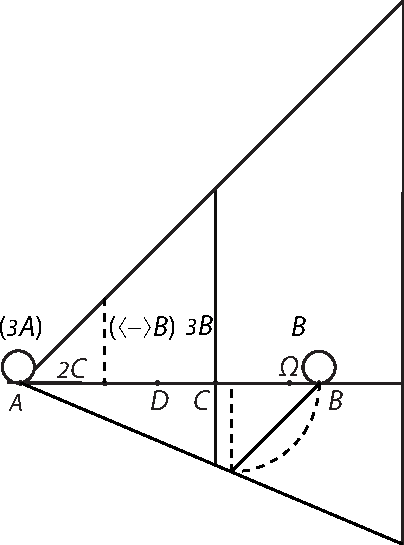
\includegraphics[width=0.4\textwidth]{%
gesamttex/edit_VIII,3/images/LH_37_05_144r_d6.pdf%
}} 
\vspace{0.5em}
\centerline{%
\lbrack\textit{Fig.~6}\rbrack%
}
% \newpage%
\vspace{1.0em}
%
%%%%%%%%%%%%%%%%%%%%%%%%%%%%%%%%
\pstart\noindent
%
%
$\begin{array}{cc}
b&a\\(A)C&(B)C.\\x&\displaystyle\frac{b}{c}x
\end{array}$
%
$\displaystyle\frac{AC}{BC} \sqcap \displaystyle\frac{b}{a} \sqcap \displaystyle\frac{{\scriptstyle \textit{2}}A{\scriptstyle \textit{2}}C}{{\scriptstyle \textit{2}}B{\scriptstyle \textit{2}}C}\, \sqcap  % doublefrac!
\edlabel{37_05_144r_2a}%
\displaystyle\doublefrac{x}{\displaystyle\frac{a}{b}x}$.%
\edtext{}{% NEUER ABSATZ UND VARIANTEN – Rechnung
{\xxref%
{37_05_144r_2a}{37_05_144r_2b}}%
\lemma{$\displaystyle\protect\doublefrac{x}{\displaystyle\frac{a}{b}x}$.}% 
\Bfootnote{%
\textit{(1)}~\textit{AC} sit \textit{x} et \textit{BC} %
\textit{(2)}~\textit{{\scriptsize3}A{\scriptsize2}C} sit \textit{x} et \textit{{\scriptsize2}B{\scriptsize2}C} %
\textit{L}%
}}%
\pend
%
\pstart \noindent
%
\textit{{\scriptsize3}A{\scriptsize2}C} sit \textit{x} et \textit{{\scriptsize2}B{\scriptsize2}C}%
\edlabel{37_05_144r_2b}
%
sit $\displaystyle\frac{a}{b}x$. Et 
sit $CD \;\sqcap\; \edtext{d \;\sqcap\; D{\scriptstyle \textit{2}}C$. Erit $\textit{D{\scriptsize 3}A}}{%
\lemma{$d \;\sqcap$}%
\Bfootnote{%
\textit{(1)}~\textit{D}(\textit{C}) %
\textit{(2)}~\textit{D{\scriptsize 2}C}. Erit  %
\textit{(a)}~\textit{D}(\textit{A})  %
\textit{(b)}~\textit{D{\scriptsize 3}A}
\textit{L}%
}}%
%
\;\sqcap \underset{\displaystyle D{\scriptstyle \textit{2}}C}{\displaystyle d} + \overset{\displaystyle{\scriptstyle \textit{3}}A{\scriptstyle \textit{2}}C}{\displaystyle x}$.  
%
Et jam $\overset{\displaystyle d}{D{\scriptstyle \textit{3}}(B)} \edtext{\smallfrown b,,+D{\scriptstyle \textit{3}}(A)a}{%
\lemma{$\smallfrown b,,+$}%
\Bfootnote{%
\textit{(1)}~\textit{D{\scriptsize 2}}(\textit{A})\textit{a} %
\textit{(2)}~\textit{D{\scriptsize 3}}(\textit{A})\textit{a}   %
~\textit{L}%
}}%
\, \sqcap \, \underset{\displaystyle g}{DBb} + \underset{\displaystyle c}{DA},a$.
%
\pend
\pstart\noindent
%
Et $D{\scriptstyle \textit{2}}(B) \sqcap\; \leibdashv\begin{array}{l}D{\scriptstyle \textit{2}}C\\d\end{array}\leibvdash\; 
%
\edlabel{37_05_144r_3a}%
\edtext{}{% NEUER ABSATZ UND VARIANTEN – Rechnung
{\xxref%
{37_05_144r_3a}{37_05_144r_3b}}%
\lemma{}%
\Bfootnote{%
$\underbrace{{\scriptstyle \textit{3}}B{\scriptstyle \textit{2}}C}_{\displaystyle \frac{a}{b}x}$. \textbar\ Vel $ 2{\scriptstyle \textit{2}}(B) \sqcap \displaystyle\frac{b}{a}x -d $ \textit{gestr.}~\textbar\ Ergo~%
\textit{L}%
}}%
\underbrace{{\scriptstyle \textit{3}}B{\scriptstyle \textit{2}}C}_{\displaystyle \frac{a}{b}x}$.
\pend
%
\pstart\noindent
Ergo%
\edlabel{37_05_144r_3b}
% 
$da+xa\;\leibdashv\; db\;\leibvdash\; ax \;\sqcap\; ac+bg$.\rule[0cm]{0mm}{12pt}%
%%
\pend
\pstart\noindent
%
Si $\leibvdash$ sit $-$ fiet $\underset{\displaystyle -c}{+d} \smallfrown a \, \sqcap\, \underset{\displaystyle -d}{+g} \smallfrown b$.
Ergo
$\displaystyle\frac{a}{b} \sqcap \displaystyle\frac{g-d}{d - c}$ seu $\displaystyle\frac{BC}{AC} \sqcap \displaystyle\frac{CB}{-A{\scriptstyle \textit{2}}C}$ si sit \textit{D} inter \textit{A} et \textit{C}.  
%
Sed si \textit{C} inter \textit{D} et \textit{A} tunc fiet $\displaystyle \frac{BC}{AC} \sqcap \displaystyle\frac{\varOmega B}{AC}$ quae absurda.\rule[0cm]{0mm}{16pt} 
%
Itaque faciemus 
$da + xa - db + xa \,\sqcap\, ac + bg$ seu\rule[0cm]{0mm}{16pt}
%
$x \,\sqcap\, \overline{b-a \smallfrown d} + \displaystyle\frac{ac+bg}{2a}$ seu $x \, \sqcap \, \displaystyle\frac{bd}{2a} + \displaystyle\frac{c-d}{2} + \displaystyle\frac{bg}{2a}$.
\pend
\count\Bfootins=1200%
\count\Afootins=1200%
\count\Cfootins=1200